\subsection{Affichage des rapports}

Dans un premier temps, nous avons vérifié le fonctionnement du système de lecture du journal grâce à un script simple exécuté en console, puis nous avons travaillé sur un système de construction de pages HTML.

\subsubsection{Architecture de l’affichage}

L’affichage est réalisé grâce à un ensemble de classes héritant de la classe abstraite \classe{Page} (un diagramme recensant ces classes est fourni en annexe), ce qui permet d’uniformiser les comportements en les intégrant à une base commune, stockée dans un fichier \texttt{template.php}.

La construction de l’interface est effectuée en deux étapes, exécutées immédiatement l’une après l’autre dans le fichier \texttt{index.php} : l’object \classe{Page} est instancié ; il stocke les paramètres du constructeur — la configuration et les paramètres de la requête — puis appelle la méthode \texttt{build}, définie par les sous-classes. Cette méthode a pour rôle la récupération des données à afficher. Dans le cas ou l’exécution de cette méthode lève une exception, la page construit un objet \classe{ExceptionPage} qui affichera l’exception.

La seconde étape est l’envoi des données à l’utilisateur, qui a lieu lors de l’appel de la méthode \texttt{display}. Celle-ci consiste en l’inclusion du fichier \texttt{template.php} ou, le cas échéant, en la délégation à la méthode \texttt{display} de l’objet \classe{ExceptionPage} créé. Le fichier \texttt{template.php}, une fois inclus, se comporte comme une partie de la méthode \texttt{build} et accède aux deux méthodes abstraite de la classe \classe{Page}, \texttt{getContent} et \texttt{getTitle}, qui retournent respectivement le contenu de la page (chaîne de caractère contenant du HTML partiel sans balise orpheline) et son titre (chaîne de caractères). Ces deux méthodes se contentent d’effectuer le formatage des données acquises précédemment et son supposées ne pas lever d’exception.

La construction de la page dans un fichier unique \texttt{template.php} et l’utilisation des méthodes statiques de la classe \classe{Page} permettent une uniformisation aisée des pages et une modification rapide.

\subsubsection{Contextes}

Pour filtrer les listes d’appels, nous avons défini la notion de contexte. Un contexte est une collection par définition de comptes sur des serveurs quelconques. Les classes représentant un contexte implémente l’interface \classe{Context}, qui définit une méthode \texttt{contains} permettant de déterminer si un compte respecte la définition reconnaissant les éléments du contexte. Cette structure ne permet pas d’extraire une liste de tous les comptes du contexte, mais a l’avantage de pouvoir représenter un contexte inconnu, par exemple un serveur distant.

Nous avons eu besoin de quatre contextes :
\begin{itemize}
	\item \classe{Account} — un compte est un contexte ne reconnaissant que lui-même, ce qui nous permet de filtrer une liste d’appels pour présenter tous les appels concernant un unique compte ;
	\item \classe{AccountGroup} — nous avons laissé la possibilité de configurer des groupes de comptes sur le serveur dont les journaux sont traités, il s’agit du seul contexte défini par ses membres, dans le fichier de configuration ;
	\item \classe{AccountDomain} — un contexte de domaine reconnaît tous les identifiants de comptes dans le domaine (sans condition de validité du compte) ;
	\item \classe{Universe} — le contexte universel permet de clore des listes de filtres ou de représenter un filtrage nul.
\end{itemize}

\subsubsection{Affichage du journal}

Pour l’affichage des journaux, nous avons créé une classe abstraite \classe{LogPage}, descendante de \classe{Page}, récupère une liste d’appels \classe{CallList} et la formate pour l’affichage. La récupération de la liste d’appels est implémentée \textit{via} une méthode \texttt{prepareLog} qui gère la sélection de la période, mais délègue le filtrage des appels aux sous-classes \textit{via} un \classe{Contexte}.

\begin{figure}
\begin{center}
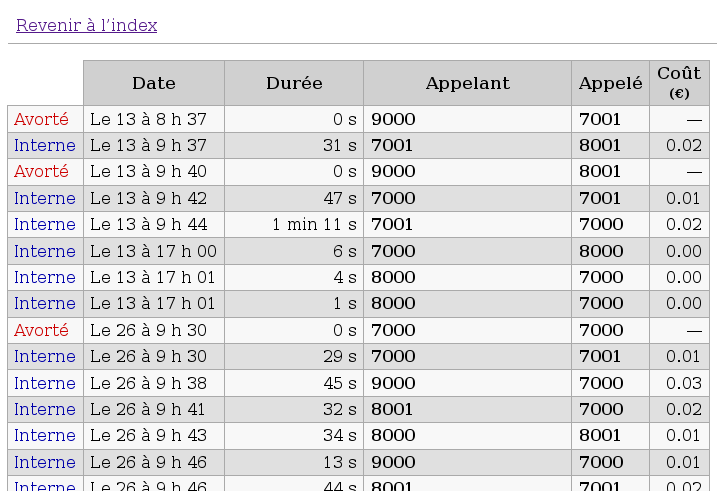
\includegraphics[width=10cm]{images/journal-global.png}
\end{center}
\label{imgjournal}
\caption{Rendu du journal global du serveur pour une série de tests}
\end{figure}

Suite à une demande de M. \nom{Laurencot}, nous avons dû ajouter à ce journal une indication des prix pour chaque appel (voir \cref{imgjournal}). Cela nous a incité à créer une classe dédiée à la gestion des prix, \classe{PriceFilters}, car les prix étaient alors gérés directement par la classe \classe{InvoicePage}.

\subsubsection{Affichage des factures}

\begin{figure}
\begin{center}
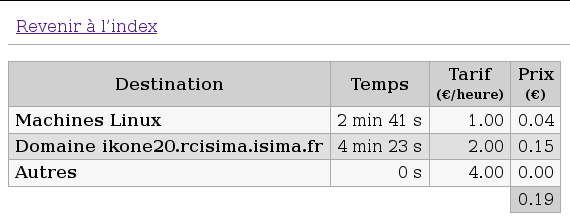
\includegraphics[width=10cm]{images/facture.png}
\end{center}
\label{imgfacture}
\caption{Rendu d’une facture}
\end{figure}

